\documentclass[12pt]{extarticle}
\usepackage{import}
\import{../}{QuantumCommands}

\usepackage{tikz-feynman}
\tikzfeynmanset{compat=1.0.0} 
\usepackage{subcaption}
\usepackage{float}
\floatplacement{figure}{H}

\begin{document}
\atitle{2}
 
\section*{Problem 1.}
Consider the non-relativistic theory with $\epsilon_p = \frac{p^2}{2m}$ and $\ket{q} = \frac{1}{\sqrt{2 \pi}} \int \d{p} e^{-ipq} \ket{p}$ and field operators,
\[ \field(t, x) = \frac{1}{\sqrt{2 \pi}} \int \d{p} \: e^{ipx - i \epsilon_p t} \: \a_p \quad \quad \dfield(t, x) = \frac{1}{\sqrt{2 \pi}} \int \d{p} e^{- i px + i \epsilon_p t} \: \adag_p\]
\subsection*{1.1}
Define the operators, 
\[ \hat{N} = \int \d{p} \adag_p \a_p \quad \quad \hat{P} = \int \d{p}  p \: \adag_p \a_p \quad \quad \hat{H} = \int \d{p} \: \epsilon_p \: \adag_p \a_p \]
Consider the commutators,
\begin{align*}
[\hat{N}, \a_p] & = \int \d{p'} \: [\adag_{p'} \a_{p'}, \a_p] = - \int \d{p'} \: \a_{p'} \delta(p' - p) = - \a_p \\
[\hat{N}, \adag_p] & = \int \d{p'} \: [\adag_{p'} \a_{p'}, \adag_p] = \int \d{p'} \: \adag_{p'} \delta(p' - p) = \adag_p
\end{align*}
Therefore, $\adag_p$ and $\a_p$ increase/decrease the eigenvalue $\hat{N}$ by $1$ which gives $\hat{N}$ the interpretation of the number of particles because the vacuum has zero $\hat{N}$ by definition. Likewise,
\begin{align*}
[\hat{P}, \a_p] & = \int \d{p'} p' \: [\adag_{p'} \a_{p'}, \a_p] = - \int \d{p'} p' \: \a_{p'} \delta(p' - p) = -p \: \a_p \\
[\hat{P}, \adag_p] & = \int \d{p'} \: p' \: [\adag_{p'} \a_{p'}, \adag_p] = \int \d{p'} \: p' \: \adag_{p'} \delta(p' - p) = p \: \adag_p
\end{align*}
Thus, $\adag_p$ increases the eigenvalue of $\hat{P}$ by $p$ which has the interpretation of $\adag_p$ as creating a particle with momentum $p$ and $\hat{P}$ counting the total momentum. Similarly, $\a_p$ destroys a particle with momentum $p$ and thus decreases $\hat{P}$ by $p$. Finally,
\begin{align*}
[\hat{H}, \a_p] & = \int \d{p'} \: \epsilon_{p'} \: [\adag_{p'} \a_{p'}, \a_p] = - \int \d{p'} \: \epsilon_{p'} \: \a_{p'} \delta(p' - p) = -\epsilon_{p} \: \a_p \\
[\hat{H}, \adag_p] & = \int \d{p'} \: \epsilon_{p'} \: [\adag_{p'} \a_{p'}, \adag_p] = \int \d{p'} \: \epsilon_{p'} \: \adag_{p'} \delta(p' - p) = \epsilon_{p} \: \adag_p
\end{align*}
sp $\adag_p$ increases the eigenvalue of $\hat{P}$ by $\epsilon_p$ which has the interpretation of $\adag_p$ as creating a particle with energy $\epsilon_p$ and $\hat{H}$ counting the total momentum. Similarly, $\a_p$ destroys a particle with energy $p$ and thus decreases $\hat{H}$ by $\epsilon_p$.
\subsection*{1.2}
\begin{align*}
i \partial_t \field(t, x) & = \frac{i}{\sqrt{2 \pi}} \int \d{p} \: (- i \epsilon_p) e^{i px - i \epsilon_p t} \: \a_p  = \frac{1}{\sqrt{2 \pi}} \int \d{p} \: \epsilon_p \: e^{i px - i \epsilon_p t} \: \a_p 
\\
[\field(t, x), \hamilt] & = \frac{1}{\sqrt{2 \pi}} \int \d{p'} \d{p} \: e^{i p' x - i \epsilon_{p'} t} \: [\a_{p'},  \epsilon_p \: \adag_p \a_p] = \frac{1}{\sqrt{2 \pi}} \int \d{p'} \d{p} \:  \epsilon_p \: e^{i p' x - i \epsilon_{p'} t} \: \a_p \: \delta(p' - p)
\\
& = \frac{1}{\sqrt{2 \pi}} \int \d{p} \: \epsilon_p \: e^{i p x - i \epsilon_p t} \: \a_p 
\end{align*}
Therefore,
\[ i \partial_t \field(t, x) = [\field(t, x), \hamilt] \] \bigskip \\
Similarly,
\begin{align*}
i \partial_x \field(t, x) & = \frac{i}{\sqrt{2 \pi}} \int \d{p} \: (i p) e^{i px - i \epsilon_p t} \: \a_p  = - \frac{1}{\sqrt{2 \pi}} \int \d{p} \: p \: e^{i px - i \epsilon_p t} \: \a_p 
\\
[\hat{P}, \field(t, x)] & = \frac{1}{\sqrt{2 \pi}} \int \d{p} \d{p'} \: e^{i p' x - i \epsilon_{p'} t} \: [p \: \adag_p \a_p, \a_{p'}] = - \frac{1}{\sqrt{2 \pi}} \int \d{p} \d{p'} \: p \: e^{i p' x - i \epsilon_{p'} t} \: \a_p \: \delta(p' - p)
\\
& = - \frac{1}{\sqrt{2 \pi}} \int \d{p} \: p \: e^{i p x - i \epsilon_p t} \: \a_p 
\end{align*}
Therefore,
\[ i \partial_x \field(t, x) = [\hat{P}, \field(t, x)] \] \bigskip \\
The time evolution of these operators is equivalent to,
\[ \field(t, x) = e^{i \hamilt t - i \hat{P} x} \field(0, 0) e^{- i \hamilt t + i \hat{P} x} \] 
This equation can be checked in two ways. First, this time evolution satisfies the above differential equations because,
\begin{align*}
\partial_t \field(t, x) & = i \hamilt e^{i \hamilt t - i \hat{P} x} \field(0, 0) e^{- i \hamilt t + i \hat{P} x} - e^{i \hamilt t - i \hat{P} x} \field(0, 0) e^{- i \hamilt t + i \hat{P} x} i \hamilt = i [\hamilt, e^{i \hamilt t - i \hat{P} x} \field(0, 0) e^{- i \hamilt t + i \hat{P} x}] 
\\
& = i [\hamilt, \field(t, x)
\\
\partial_t \field(t, x) & = -i \hat{P} e^{i \hamilt t - i \hat{P} x} \field(0, 0) e^{- i \hamilt t + i \hat{P} x} + e^{i \hamilt t - i \hat{P} x} \field(0, 0) e^{- i \hamilt t + i \hat{P} x} i \hat{P} = - i [\hat{P}, e^{i \hamilt t - i \hat{P} x} \field(0, 0) e^{- i \hamilt t + i \hat{P} x}] 
\\
& = - i [\hat{P}, \field(t, x)
\end{align*}
which hold because $[\hamilt, \hat{P}] = 0$. 
On the other hand,
\begin{align*}
[\hamilt, \a_p] = - \epsilon_p \: \a_p \quad & \quad [\hamilt, \adag_p] = \epsilon_p \: \adag_p 
\\
[\hat{P}, \a_p] = - p \: \a_p \quad & \quad [\hat{P}, \adag_p] = p \: \adag_p 
\end{align*}
so we have the relations,
\begin{align*}
e^{i \hamilt t - i \hat{P} x} \a_p e^{- i \hamilt t + i \hat{P} x} & = \a_p e^{i p x - i \epsilon_p t} 
\\
e^{i \hamilt t - i \hat{P} x} \adag_p e^{- i \hamilt t + i \hat{P} x} & = \adag_p e^{- i p x + i \epsilon_p t}
\end{align*}
Therefore,
\begin{align*}
e^{i \hamilt t - i \hat{P} x} \field(0, 0) e^{- i \hamilt t + i \hat{P} x} & = \a_p e^{i p x - i \epsilon_p t} = \frac{1}{\sqrt{2 \pi}} \int \d{p}  e^{i \hamilt t - i \hat{P} x} \a_p e^{- i \hamilt t + i \hat{P} x} = \frac{1}{\sqrt{2 \pi}} \int \d{p} e^{i p x - i \epsilon_p t} \: \a_p = \field(t, x) 
\end{align*}
\subsection*{1.3}
The equal-time commutators are,
\begin{align*}
[ \field(t, x), \field(t, x')] & = \frac{1}{2\pi} \int \d{p} \d{p'} \: e^{i p x - i \epsilon_p t} [\a_p, \a_{p'}] e^{i p' x' - i \epsilon_{p'} t} = 0 \\
[ \field(t, x), \dfield(t, x')] & = \frac{1}{2\pi} \int \d{p} \d{p'} \: e^{i p x - i \epsilon_p t} [\a_p, \adag_{p'}] e^{-i p' x' + i \epsilon_{p'} t} = \frac{1}{2\pi} \int \d{p} \d{p'} \: e^{i p x - i p' x' - i (\epsilon_p - \epsilon_{p'}) t} \delta(p - p')
\\
& = \frac{1}{2\pi} \int \d{p} \: e^{i p (x - x')} = \delta(x - x')
\end{align*}
\subsection*{1.4}
\begin{align*}
\dfield(t, x) \ket{0} = \frac{1}{\sqrt{2 \pi}} \int \d{p} \: e^{i p x - i\epsilon_p t} \: \a_p \ket{0} =  \frac{1}{\sqrt{2 \pi}} \int \d{p} \: e^{i p x - i\epsilon_p t} \: \ket{p} = \ket{x, t}
\end{align*}
so $\dfield(t, x)$ creates a particle at $(t, x)$. \bigskip\\
Furthermore, expanding the integral,
\begin{align*}
\int \d{x} \: \dfield(t, x) \left( - \frac{1}{2m} \partial_x^2\right) \field(t, x) & = \frac{1}{2\pi} \int \d{x} \: \d{p} \d{p'} \: e^{- i p x + i \epsilon_p t} \: \adag_p \left(- \frac{1}{2 m} ( i p')^2 \right) e^{i p' x - i \epsilon_{p'} t} \: \a_{p'} 
\\
& = \frac{1}{2\pi} \int \d{p} \d{p'} \: \frac{(p')^2}{2m} \: \adag_p \a_{p'}  \int \d{x} \: e^{i (p' - p) x - i (\epsilon_{p'} - \epsilon_{p}) t}
\\
& = \frac{1}{2\pi} \int \d{p} \d{p'} \: \frac{(p')^2}{2m}  \: \adag_p \a_{p'} \: e^{- i (\epsilon_{p'} - \epsilon_{p}) t} \delta(p' - p)
\\
& = \int \d{p} \: \frac{p^2}{2m}  \: \adag_p \a_{p} = \int \d{p} \: \epsilon_p \: \adag_p \a_{p} = \hamilt
\end{align*}
Therefore,
\[\hamilt = \int \d{x} \: \dfield(t, x) \left( - \frac{1}{2m} \partial_x^2\right) \field(t, x)\]
\bigskip\\
Similarly,
\begin{align*}
\int \d{x} \: \dfield(t, x) \field(t, x) & = \frac{1}{2\pi} \int \d{x} \: \d{p} \d{p'} \: e^{- i p x + i \epsilon_p t} \: \adag_p  e^{i p' x - i \epsilon_{p'} t} \: \a_{p'} 
\\
& = \frac{1}{2\pi} \int \d{p} \d{p'} \: \adag_p \a_{p'}  \int \d{x} \: e^{i (p' - p) x - i (\epsilon_{p'} - \epsilon_{p}) t}
\\
& = \frac{1}{2\pi} \int \d{p} \d{p'} \: \adag_p \a_{p'} \: e^{- i (\epsilon_{p'} - \epsilon_{p}) t} \delta(p' - p)
\\
& = \int \d{p} \: \adag_p \a_{p} = \hat{N}
\end{align*}
Therefore,
\[ \hat{N} = \int \d{x} \: \dfield(t, x) \field(t, x)\]
\bigskip\\
Similarly,
\begin{align*}
\int \d{x} \: \dfield(t, x) \left( \frac{1}{i} \partial_x\right) \field(t, x) & = \frac{1}{2\pi} \int \d{x} \: \d{p} \d{p'} \: e^{- i p x + i \epsilon_p t} \: \adag_p \: p' \: e^{i p' x - i \epsilon_{p'} t} \: \a_{p'} 
\\
& = \frac{1}{2\pi} \int \d{p} \d{p'} \: p' \: \adag_p \a_{p'}  \int \d{x} \: e^{i (p' - p) x - i (\epsilon_{p'} - \epsilon_{p}) t}
\\
& = \frac{1}{2\pi} \int \d{p} \d{p'} \: p'  \: \adag_p \a_{p'} \: e^{- i (\epsilon_{p'} - \epsilon_{p}) t} \delta(p' - p)
\\
& = \int \d{p} \: p \: \adag_p \a_{p} = \int \d{p} \: p \: \adag_p \a_{p} = \hat{P}
\end{align*}
Therefore,
\[\hat{P} = \int \d{x} \: \dfield(t, x) \left( \frac{1}{i} \partial_x\right) \field(t, x)\]
\subsection*{1.5}
Define the wavefunction,
\begin{align*}
\psi_p(t, x) & = \bra{0} \field(t, x) \ket{p} = \int \d{p'} \: e^{i p' x - i \epsilon_{p'} t} \bra{0} \a_{p'} \adag_p \ket{0} \int \d{p'} \: e^{i p' x - i \epsilon_{p'} t} \bra{0} [\a_{p'},  \adag_p] \ket{0} 
\\
& = \int \d{p'}  e^{i p' x - i \epsilon_{p'} t} \delta(p' - p) = e^{i p x - i \epsilon_p t}
\end{align*}
This function clearly satisfies the Schrödinger equation, 
\[ i \partial_t \psi_p(t, x) = \epsilon_p \: e^{i p x - i \epsilon_p t} = \frac{p^2}{2m} e^{i p x - i \epsilon_p t} = - \frac{1}{2m} \partial_x^2 \psi_p(t, x)\]
However, any single particle state can be written as a superposition of definite momentum states,
\[ \ket{\psi} = \frac{1}{\sqrt{2 \pi}} \int \d{p} \tilde{\psi}(p) \ket{p} = \frac{1}{\sqrt{2 \pi}} \int \d{p} \tilde{\psi}(p) \a_p \ket{0} \]
Therefore,
\[ \psi(t, x) = \bra{0} \field(t, x) \ket{\psi} = \frac{1}{\sqrt{2 \pi}} \int \d{p} \tilde{\psi}(p) \bra{0} \field(t, x) \ket{p} = \frac{1}{\sqrt{2 \pi}} \int \d{p} \tilde{\psi}(p) \psi_p(t, x) \]
But each $\psi_p(t, x)$ individually satisfies the Schrödinger equation so, because the Schrödinger equation is linear, any linear combination is also a solution. Therefore, $\psi(t, x) = \bra{0} \field(t, x) \ket{\psi}$ satisfies the Schrödinger equation. \bigskip \\
Alternatively, first calculate the commutator in the Heisenberg equations of motion,
\begin{align*}
i \partial_t \field(t, x) & = [\field(t, x), \hamilt] = \int \d{x'} [ \field(t, x), \dfield(t, x') \left( - \frac{1}{2m} \partial_{x}^2 \right) \field(t, x')]
\\
& = \int \d{x'} \delta(x - x') \left( - \frac{1}{2m} \partial_{x}^2 \right) \field(t, x') = \left( - \frac{1}{2m} \partial_{x}^2 \right) \field(t, x)
\end{align*} 
so the field operator $\field(t, x)$ satisfies the Schrödinger equation,
\[ i \partial_t \field(t, x) = - \frac{1}{2m} \partial_{x}^2 \field(t, x)\]
\begin{align*}
i \partial_t \phi(t, x) & = \bra{0} i \partial_t \field(t, x) \ket{\psi} = \bra{0} [\field(t, x), \hamilt] \ket{\psi}
\\
& = \bra{0} \left( - \frac{1}{2m} \partial_{x}^2 \right) \field(t, x) \ket{\psi} 
= - \frac{1}{2m} \partial_x^2 \bra{0} \field(t, x) \ket{\psi} = - \frac{1}{2m} \partial_x^2 \psi(t, x)
\end{align*} 
Therefore,
\[ i \partial_t \psi(t, x) = - \frac{1}{2m} \partial_x^2 \psi(t, x)\]
so $\psi(t, x)$ satisfies the Schrödinger equation. 
\subsection*{1.6}
Define the two particle wavefunction,
\[ \psi(t, x, y) = \bra{0} \field(t, x) \field(t, y) \ket{\psi}\]
Now, consider the time dependence of $\psi(t, x, y)$,
\begin{align*}
i \partial_t \psi(t, x, y) & = \bra{0} i \partial_t \field(t, x) \field(t, y) + \field(t, x) i \partial_t \field(t, y) \ket{\psi} = - \frac{1}{2m} \bra{0} \partial_x^2 \field(t, x) \field(t, y) + \field(t, x) \partial_y^2 \field(t, y) \ket{\psi}
\\
& = - \frac{1}{2m} \bra{0} \partial_x^2 \field(t, x) \field(t, y) \ket{\psi} - \frac{1}{2m} \bra{0} \field(t, x) \partial_y^2 \field(t, y) \ket{\psi} 
\\
& = - \frac{1}{2m} \partial_x^2 \bra{0} \field(t, x) \field(t, y) \ket{\psi} - \frac{1}{2m} \partial_y^2 \bra{0} \field(t, x) \field(t, y) \ket{\psi}
\\
& = - \frac{1}{2m} \partial_x^2 \psi(t, x, y) - \frac{1}{2m} \partial_y^2 \psi(t, x, y)
\end{align*}
Therefore, $\psi(t, x, y)$ satisfies the two-particle Schrödinger equation,
\[ i \partial_t \psi(t, x, y) = - \frac{1}{2m} \left( \partial_x^2 + \partial_y^2 \right) \psi(t, x, y)\]
\subsection*{1.7}

Let $A(t')$ be a Hermitian operator representing some physical observable and let $\ket{a, t'}$ be a basis of eigenvectors of $\hat{A}(t')$ with $a$ ranging over the spectrum. Using the fact that $\dfield$ creates a particle at $(t, x)$ i.e. $\dfield(t, x) \ket{0} = \ket{q, t}$ we can interpret the quantitiy, 
\[ |\bra{0} \field(t, x) \ket{a, t'} |^2 = | \inner{q, t}{a, t'} |^2 \]
For $t > t'$,
\[ |\bra{0} \field(t, x) \ket{a, t'} |^2 = | \inner{q, t}{a, t'} |^2 = | \bra{q} e^{- i \hamilt (t - t')} \ket{a} |^2 \]
which is the probability for the state with definite value $a$ of the observable $\hat{A}$ to evolve into the state with a single particle located at $x$ after a time $t - t'$. \bigskip\\
Likewise, for $t < t'$,
\[ |\bra{0} \field(t, x) \ket{a, t'} |^2 = | \inner{a, t'}{t, x} |^2 = | \bra{a} e^{- i \hamilt (t' - t)} \ket{q} |^2 \]
which is the probability for the state with a single particle located at $x$ to evolve into the state with definite value $a$ of the observable $\hat{A}$ after a time $t' - t$. \bigskip\\

\subsection*{1.8}
Define the non-relativistic propagator, 
\begin{align*}
K(t,x|t',x') & = \bra{0} \bf{T} \: \field(t, x) \: \dfield(t', x') \ket{0}
\\
& = \frac{1}{2 \pi} \int \d{p} \d{p'} e^{i p x - i \epsilon_p t}  \: \bra{0} \bf{T} \: \a_p \adag_{p'} \ket{0} \: e^{- i p' x' + i \epsilon_{p'} t'} 
\\
& = \frac{1}{2 \pi} \int \d{p} \d{p'} e^{i p x - i p' x' - i \epsilon_p t + i \epsilon_{p'} t'} \cdot
\begin{cases}
\delta(p - p') & t > t'\\
0  & t < t'
\end{cases}
\\
& = 
\begin{cases}
\frac{1}{2 \pi} \int \d{p} e^{i p (x - x') - i \epsilon_p (t - t')} & t > t' \\
0 & t < t'
\end{cases}
\end{align*}
Consider the integral,
\begin{align*}
\frac{1}{2 \pi} \int \d{p} e^{i p (x - x') - i \epsilon_p (t - t')} & = \frac{1}{2 \pi} \int \d{p} e^{i p (x - x') - i \frac{p^2}{2m} (t - t')}
\\
& = \sqrt{\frac{m}{2 \pi i(t - t')}} \: e^{\frac{i m (x - x')^2}{2 (t - t')}}
\end{align*}
Therefore, the propagator is given by,
\[ K(t, x | t', x') = 
\begin{cases}
\sqrt{\frac{m}{2 \pi i(t - t')}} \: e^{\frac{i m (x - x')^2}{2 (t - t')}}  & t > t' \\
0 & t < t'
\end{cases}
\]
The propagator can be interpreted as, 
\[K(t, x| t', x') = \bra{0} \bf{T} \: \field(t, x) \: \dfield(t', x') \ket{0}
=
\begin{cases}
\inner{x, t}{x', t'} & t > t'\\
0 & t < t'
\end{cases}
\]
which is the amplitude for a particle at $(x', t')$ to propagate to $(x, t)$ i.e. the amplitude for a particle created at $(x', t')$ to be measured at position $x$ at time $t$. \bigskip \\
To calculate the four-point function,
\[\bra{0} \bf{T} \: \field(t_1, x_1) \field(t_2, x_2) \dfield(t_3, x_3) \dfield(t_4, x_4) \ket{0}\]
we first calculate the (unequal-time) commutator between the fields,
\begin{align*}
[\field(t, x), \field(t', x')] & = 0 \\
[\field(t, x), \dfield(t', x')] & = \frac{1}{2 \pi} \int \d{p} \d{p'} e^{i p x - i \epsilon_p t}  \: [\a_p, \adag_{p'}] \: e^{- i p' x' + i \epsilon_{p'} t'} 
\\
& = \frac{1}{2 \pi} \int \d{p} \d{p'} e^{i p x - i \epsilon_p t}  \: \delta(p - p') \: e^{- i p' x' + i \epsilon_{p'} t'} 
\\
& = \frac{1}{2 \pi} \int \d{p} e^{i p (x - x') - i \epsilon_p (t - t')} = \sqrt{\frac{m}{2 \pi i(t - t')}} \: e^{\frac{i m (x - x')^2}{2 (t - t')}}
\end{align*}
I define a commutator under the time ordering symbol to be the ordinary commutator if the operators are written in correctly time ordered form and zero if time ordering would put the operators in the opposite order. That is,
\[ \bf{T} AB = \bf{T} ([A, B]) + BA  \]
Clearly, under this definition,
\[ \bf{T} [\field(t, x), \dfield(t', x')] = K(t, x | t', x') \]
Finally, we calculate the four-point function,
\begin{align*}
\bra{0} & \bf{T} \: \field(t_1, x_1) \field(t_2, x_2) \dfield(t_3, x_3) \dfield(t_4, x_4) \ket{0} 
\\
& = \bra{0} \bf{T} \: \field(t_1, x_1) [\field(t_2, x_2), \dfield(t_3, x_3)] \dfield(t_4, x_4) \ket{0} + \bra{0} \bf{T} \: \field(t_1, x_1) \dfield(t_3, x_3) \field(t_2, x_2) \dfield(t_4, x_4) \ket{0}
\\
& = \bra{0} \bf{T} \: \field(t_1, x_1) \dfield(t_4, x_4) \ket{0} K(t_2, x_2 | t_3 x_3) + \bra{0} \bf{T} \: \field(t_1, x_1) \dfield(t_3, x_3) \field(t_2, x_2) \dfield(t_4, x_4) \ket{0}
\\
& = K(t_1, x_1 | t_4, x_4) K(t_2, x_2 | t_3 x_3) + \bra{0} \bf{T} \: \field(t_1, x_1) \dfield(t_3, x_3) [\field(t_2, x_2), \dfield(t_4, x_4)] \ket{0}
\\
& = K(t_1, x_1 | t_4, x_4) K(t_2, x_2 | t_3 x_3) + \bra{0} \bf{T} \: \field(t_1, x_1) \dfield(t_3, x_3) \ket{0} K(t_2, x_2 | t_4, x_4)
\\
& = K(t_1, x_1 | t_4, x_4) K(t_2, x_2 | t_3 x_3) + K(t_1, x_1 | t_3, x_3) K(t_2, x_2 | t_4, x_4) 
\end{align*}
Therefore, the four-point function can be expressed in terms of $K$-propagators as,
\[\bra{0} \bf{T} \: \field(t_1, x_1) \field(t_2, x_2) \dfield(t_3, x_3) \dfield(t_4, x_4) \ket{0} = K(t_1, x_1 | t_4, x_4) K(t_2, x_2 | t_3 x_3) + K(t_1, x_1 | t_3, x_3) K(t_2, x_2 | t_4, x_4) \]
This four-point function corresponds to the Feynman diagrams of the two possible contractions on four points respecting ordering, 

\begin{figure}
\centering
\begin{minipage}{.5\textwidth}
  \centering
  
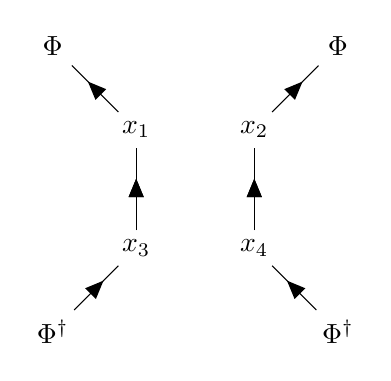
\begin{tikzpicture}
\begin{feynman}
\vertex (i1) {\( \Phi^\dagger \)};
\vertex [above right=of i1] (a) {\(x_3\)};
\vertex [above =of a] (b) {\(x_1\)};
\vertex [above left =of b] (o1) { \(\Phi\) };
\vertex [right =of a] (c) {\(x_4\)};
\vertex [right =of b] (d) {\(x_2\)};
\vertex [above right =of d] (o2) { \(\Phi\) };
\vertex [below right =of c] (i2) { \(\Phi^\dagger\) };
\diagram* {
(i1) -- [fermion] (a) -- [fermion] (b),
(a) -- [fermion] (b) -- [fermion] (o1),
(i2) -- [fermion] (c) -- [fermion] (d),
(c) -- [fermion] (d) -- [fermion] (o2),
};
\end{feynman}
\end{tikzpicture}

\end{minipage}%
\begin{minipage}{.5\textwidth}
  \centering
  
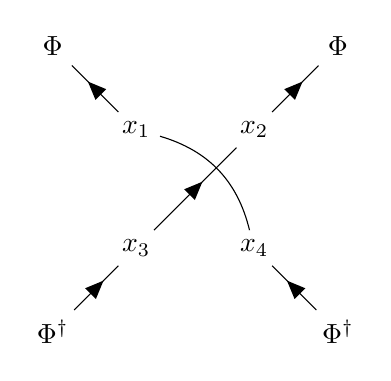
\begin{tikzpicture}
\begin{feynman}
\vertex (i1) {\( \Phi^\dagger \)};
\vertex [above right=of i1] (a) {\(x_3\)};
\vertex [above =of a] (b) {\(x_1\)};
\vertex [above left =of b] (o1) { \(\Phi\) };
\vertex [right =of a] (c) {\(x_4\)};
\vertex [right =of b] (d) {\(x_2\)};
\vertex [above right =of d] (o2) { \(\Phi\) };
\vertex [below right =of c] (i2) { \(\Phi^\dagger\) };
\diagram* {
(i1) -- [fermion] (a),
(a) -- [fermion] (d) -- [fermion] (o2),
(i2) -- [fermion] (c),
(c) -- [bend right] (b) -- [fermion] (o1),
};
\end{feynman}
\end{tikzpicture}  
  
\end{minipage}
\end{figure}


\subsection*{1.9}
Consider the action of a nonrelativistic complex scalar field,
\[ S = \int \d{t} \d{x} \left( i \Phi^* \partial_t \Phi - \Phi^* \left(-\tfrac{1}{2m} \partial_x^2 \right) \Phi \right) \] 
with canonical momenta,
\[ \pi_{\Phi} = \pderiv{\lagrange}{(\partial_t \Phi)} = i \Phi^* \quad \quad \pi_{\Phi^*} = \pderiv{\lagrange}{(\partial_t \Phi^*)} = 0 \]
and thus a Hamiltonian,
\[ \mathcal{H} = \pi_\Phi \partial_t \Phi + \pi_{\Phi^*} \partial_t \Phi^* - \lagrange = \Phi^* \left(-\tfrac{1}{2m} \partial_x^2 \right) \Phi\]
This action is canonically quantized by promoting the fields to operators $\Phi \to \field$ and imposing the canonical commutation relation,
\[ [ \field(t, x), \hat{\pi}_{\field}(t, x')] = [\field(t, x), i\dfield(t, x')] = i \delta(x - x')\] 
Therefore,
\[ [\field(t, x), \dfield(t, x')] = \delta(x - x')\]
and the operators $\field(t, x)$ and $\dfield(t, x)$ commute with themselves. These are the commutation relations we found earlier. Furthermore, the Hamiltonian operator becomes,
\[ \hamilt = \int \d{x} \hat{\mathcal{H}} = \int \d{x} \dfield \left(-\tfrac{1}{2m} \partial_x^2 \right) \field \]
Therefore, canonical quantization of this action reproduces the nonrelativistic Hamiltonian and commutation relations. 
\subsection*{1.10}
Consider action of a relativistic scalar field is given by,
\[ \int \d{t} \d{x} \left[ \phi^* \left( - \tfrac{1}{c^2} \partial_t^2 + \partial_x^2 \right) \phi - (mc)^2 \phi^* \phi \right] \]
Let $\phi(t, x) = \tfrac{1}{\sqrt{2m}} e^{- i m c^2 t}\field(t, x)$. Then,
\begin{align*}
S & = \tfrac{1}{2m} \int \d{t} \d{x} \left[ e^{i m c^2 t} \dfield \left( - \tfrac{1}{c^2} \partial_t^2 + \partial_x^2 \right) e^{- i m c^2 t} \field - (mc)^2 \dfield \field \right]
\\
& = \tfrac{1}{2m} \int \d{t} \d{x} \left[ \dfield \left( - \tfrac{1}{c^2} \partial_t^2 + 2 i m \partial_t + (mc)^2 +  \partial_x^2 \right) \field - (mc)^2 \dfield \field \right]
\\
& = \tfrac{1}{2m} \int \d{t} \d{x} \dfield \left( - \tfrac{1}{c^2} \partial_t^2 + 2 i m \partial_t + \partial_x^2 \right) \field
\\
& = \int \d{t} \d{x} \dfield \left( - \tfrac{1}{2 m c^2} \partial_t^2 + i \partial_t + \tfrac{1}{2m} \partial_x^2 \right) \field
\\
& = \int \d{t} \d{x} \left( - \dfield \tfrac{1}{2 m c^2} \partial_t^2 \field + i \dfield  \partial_t \field - \dfield \left( - \tfrac{1}{2m} \partial_x^2 \right) \field \right)
\end{align*}
In the limit $c \to \infty$ while holding other constants finite, the term $- \dfield \tfrac{1}{2 m c^2} \partial_t^2 \field$ drops out. Thus, the action becomes,
\[ S =  \int \d{t} \d{x} \left( i \dfield  \partial_t \field - \dfield \left( - \tfrac{1}{2m} \partial_x^2 \right) \field \right)\]
which is equal to the action considered earlier. 
\subsection*{1.11}
Now consider the 3D nonrelativistic interacting field Hamiltonian,
\[ \hamilt = \int \d{^3x} \dfield(x) \left( -\tfrac{1}{2m} \nabla^2 + V(x)\right) \field(x) + \int \d{^3x} \d{^3y} \dfield(x) \dfield(y) \frac{g^2}{|x - y|} \field(x) \field(y) \]
with (equal-time) commutation relations,
\[[\field(x), \dfield(y)] = \delta^3(x - y) \quad \quad [\field(t, x), \field(t, y)] = [\dfield(t, x), \dfield(t, y)] = 0\]
These field operators are extended to time-dependent operators satisfying the Heisenberg equation,
\[ i \partial_t \field(t, x) = [\field(t, x), \hamilt] \]
First, we calculate this time evolution commutator,
\begin{align*}
[\field(t, x), \hamilt] & = \int \d{^3 x'} [\field(t, x), \dfield(t, x')] \left( -\tfrac{1}{2m} \nabla^2 + V(x')\right) \field(t, x') 
\\
& + \int \d{^3x'} \d{^3y'} [\field(t, x), \dfield(t, x') \dfield(t, y')] \frac{g^2}{|x' - y'|} \field(t, x') \field(t, y')
\\
& = \int \d{^3 x'} \delta^3(x - x') \left( -\tfrac{1}{2m} \nabla^2 + V(x')\right) \field(t, x')
\\
& + \int \d{^3x'} \d{^3y'} \left( \delta^3(x - x') \dfield(t, y') + \dfield(t, x') \delta^3(x - y') \right) \frac{g^2}{|x' - y'|} \field(t, x') \field(t, y')
\\
& = \left( -\tfrac{1}{2m} \nabla^2 + V(x)\right) \field(t, x)
\\
& + \int \d{^3y'} \dfield(t, y') \frac{g^2}{|x - y'|} \field(t, x) \field(t, y') + \int \d{^3x'}  \dfield(t, x') \frac{g^2}{|x' - x|} \field(t, x') \field(t, x)
\\
& = \left( -\tfrac{1}{2m} \nabla^2 + V(x)\right) \field(t, x) + \int \d{^3x'}  \dfield(t, x') \frac{2 g^2}{|x' - x|} \field(t, x') \field(t, x)
\end{align*}
Consider the two particle wavefunction of a state $\ket{\psi}$,
\[ \psi(t, x, y) = \bra{0} \field(t, x) \field(t, y) \ket{\psi} \]
which has time dependence,
\begin{align*}
i \partial_t \psi(t, x, y) & = \bra{0} i \partial_t \field(t, x) \field(t, y) \ket{\psi} + \bra{0} \field(t, x)  i \partial_t \field(t, y) \ket{\psi}
\\
& = \bra{0} \left( -\tfrac{1}{2m} \nabla^2 + V(x)\right) \field(t, x) \field(t, y) \ket{\psi} + \int \d{^3x'}  \bra{0} \dfield(t, x') \frac{2 g^2}{|x' - x|} \field(t, x') \field(t, x) \field(t, y) \ket{\psi}
\\
& + \bra{0} \field(t, x) \left( -\tfrac{1}{2m} \nabla^2 + V(y)\right) \field(t, y) \ket{\psi} + \bra{0} \field(t, x)  \int \d{^3x'}  \dfield(t, x') \frac{2 g^2}{|x' - y|} \field(t, x') \field(t, y) \ket{\psi} 
\\
& = \left( -\tfrac{1}{2m} \nabla_x^2 + V(x)\right) \bra{0} \field(t, x) \field(t, y) \ket{\psi} + \left( -\tfrac{1}{2m} \nabla_y^2 + V(y)\right) \bra{0} \field(t, x) \field(t, y) \ket{\psi}
\\
& + \int \d{^3x'}  \bra{0} [\field(t, x), \dfield(t, x')] \frac{2 g^2}{|x' - y|} \field(t, x') \field(t, y) \ket{\psi}
\\
& = \left( -\tfrac{1}{2m} \nabla_x^2 -\tfrac{1}{2m} \nabla_y^2 + V(x) + V(y)\right) \psi(t, x, y) + \int \d{^3x'}  \bra{0} \delta^3(x - x') \frac{2 g^2}{|x' - y|} \field(t, x') \field(t, y) \ket{\psi}
\\
& = \left( -\tfrac{1}{2m} \nabla_x^2 -\tfrac{1}{2m} \nabla_y^2 + V(x) + V(y)\right) \psi(t, x, y) + \frac{2 g^2}{|x - y|}  \bra{0} \field(t, x) \field(t, y) \ket{\psi}
\\
& = \left( -\tfrac{1}{2m} \nabla_x^2 -\tfrac{1}{2m} \nabla_y^2 + V(x) + V(y)\right) \psi(t, x, y) + \frac{2 g^2}{|x - y|}  \psi(t, x, y)
\end{align*}
Therefore, the wavefunction $\psi$ satisfies 2-particle Schrödinger equation with Coulombic interaction,
\[ i \partial_t \psi(t, x, y) = \left( -\frac{1}{2m} \nabla_x^2 -\frac{1}{2m} \nabla_y^2 + V(x) + V(y) + \frac{2 g^2}{|x - y|} \right) \psi(t, x, y) \]
\section*{Problem 2.}
Consider the action for a relativistic complex scalar field,
\[ S = \int \d{t} \d{x} \left( \partial_\mu \phi^* \partial^\mu \phi - m^2 \phi^* \phi \right) \]
Using canonical quantization, we express the field as,
\begin{align*}
\phi(t, x) & = \frac{1}{\sqrt{2 \pi}} \int \d{p} \frac{1}{\sqrt{2 \epsilon_p}} \left( e^{i p x - i \epsilon_p t} \: \a_p + e^{- i p x + i \epsilon_p t} \: \bdag_p \right) 
\\
\phi^\dagger(t, x) & = \frac{1}{\sqrt{2 \pi}} \int \d{p} \frac{1}{\sqrt{2 \epsilon_p}} \left( e^{i p x - i \epsilon_p t} \: \b_p + e^{- i p x + i \epsilon_p t} \: \adag_p \right) 
\end{align*}
where $\epsilon_p = \sqrt{m^2 + p^2}$ and $[\a_p, \adag_{p'}] = [\b_p, \bdag_{p'}] = \delta(p - p')$. 
\subsection*{2.1}
Consider the canonical momenta, $\pi(t, x) = \pderiv{\lagrange}{(\partial_t \phi)} = \partial_t \phi^\dagger(t, x)$ and $\pi^\dagger(t, x) = \pderiv{\lagrange}{(\partial_t \phi^\dagger)} = \partial_t \phi(t, x)$  Expressing this in terms of creation and annihilation operators,
\begin{align*} 
\pi(t, x) & = \frac{i}{\sqrt{2 \pi}} \int \d{p} \sqrt{\frac{\epsilon_p}{2}} \left(  e^{-i p x + i \epsilon_p t} \: \adag_p - e^{i p x - i \epsilon_p t} \: \b_p\right)
\\
\pi^\dagger(t, x) & = \frac{i}{\sqrt{2 \pi}} \int \d{p} \sqrt{\frac{\epsilon_p}{2}} \left( e^{- i p x + i \epsilon_p t} \: \bdag_p - e^{i p x - i \epsilon_p t} \: \a_p \right) 
\end{align*}
Now, the commutation relations become,
\begin{align*}
[\phi(t, x), \pi(t, x')] & = \frac{i}{4\pi} \int \d{p} \d{p'} \left(e^{i p x - i \epsilon_p t - i p' x' + i \epsilon_{p'} t} [\a_p, \adag_{p'}] - e^{-i p x + i \epsilon_p t + i p' x' - i \epsilon_{p'} t} [\bdag_p, \b_{p'}] \right) 
\\
& = \frac{i}{4\pi} \int \d{p} \d{p'} \left(e^{i p x - i \epsilon_p t - i p' x' + i \epsilon_{p'} t} \delta(p - p') + e^{-i p x + i \epsilon_p t + i p' x' - i \epsilon_{p'} t} \delta(p - p') \right) 
\\
& = \frac{i}{2\pi} \int \d{p} e^{i p (x - x')} = i \delta(x  - x') 
\\
[\phi(t, x), \pi^\dagger(t, x')] & = \frac{i}{4\pi} \int \d{p} \d{p'} \left(- e^{i p x - i \epsilon_p t + i p' x' - i \epsilon_{p'} t} [\a_p, \a_{p'}] + e^{-i p x + i \epsilon_p t - i p' x' + i \epsilon_{p'} t} [\bdag_p, \bdag_{p'}] \right) = 0
\\
[\phi^\dagger(t, x), \pi(t, x')] & = [\pi^\dagger(t, x'), \phi(t, x)]^\dagger = 0
\\
[\phi^\dagger(t, x), \pi^\dagger(t, x')] & = [\pi(t, x'), \phi(t, x)]^\dagger = ( - i \delta(x - x'))^* = i \delta(x - x')
\end{align*}
Summarizing,
\begin{align*}
[\phi(t, x), \pi(t, x')] & = i \delta(x - x') \\
[\phi(t, x), \pi^\dagger(t, x')] & = 0 \\
[\phi^\dagger(t, x), \pi(t, x')] & = 0 \\
[\phi^\dagger(t, x), \pi^\dagger(t, x')] & = i \delta(x - x')
\end{align*}
\subsection*{2.2}
The Hamiltonian is given by a Legendre transformation,
\[ \mathcal{H} = \pi \partial_t \phi + \pi^\dagger \partial_t \phi^\dagger - \lagrange = \pi^\dagger \pi + \partial_x \phi^\dagger \partial_x \phi + m^2 \phi^\dagger \phi \]
Now, we calculate the full Hamiltonian,
\[ \hamilt = \int \d{x} \mathcal{H} \]
term by term,
\begin{align*}
\int & \d{x} \pi^\dagger \pi
\\
& = \int \frac{\d{x} \d{p} \d{p'}}{4 \pi} \left( \sqrt{\epsilon_p \epsilon_{p'}}  \left[ e^{i p x - i \epsilon_p t} \: \a_p - e^{- i p x + i \epsilon_p t} \: \bdag_p \right] \left[e^{-i p' x + i \epsilon_{p'} t} \: \adag_{p'} - e^{i p' x - i \epsilon_{p'} t} \: \b_{p'} \right] \right) 
\\ 
& = \int \frac{\d{x} \d{p} \d{p'}}{4 \pi} \sqrt{\epsilon_p \epsilon_{p'}} \left( \left[e^{i (\epsilon_{p'} - \epsilon_p) t} \a_p \adag_{p'} + e^{i (\epsilon_p - \epsilon_{p'}) t} \bdag_p \b_{p'} \right] e^{i (p - p') x} -
\left[e^{i (\epsilon_{p'} + \epsilon_p) t} \bdag_p \adag_{p'} + e^{-i (\epsilon_p + \epsilon_{p'}) t} \a_p \b_{p'} \right] e^{i (p + p') x} \right)
\\
& = \frac{1}{2} \int \d{p} \epsilon_p \left(\a_p \adag_{p} + \bdag_p \b_{p} -
\bdag_p \adag_{-p} e^{2 i \epsilon_p} - \a_p \b_{-p} e^{-2 i \epsilon_p} \right)
\end{align*}
Similarly,
\begin{align*}
\int & \d{x} \partial_x \phi^\dagger \partial_x \phi 
\\
& = \int \frac{\d{x} \d{p} \d{p'}}{4 \pi} \left( \frac{1}{\sqrt{\epsilon_p \epsilon_{p'}}} \: \partial_x \left[ e^{i p x - i \epsilon_p t} \: \b_p + e^{- i p x + i \epsilon_p t} \: \adag_p \right] \partial_x \left[e^{i p' x - i \epsilon_{p'} t} \: \a_{p'} + e^{- i p' x + i \epsilon_{p'} t} \: \bdag_{p'} \right]   \right) 
\\ 
& = \int \frac{\d{x} \d{p} \d{p'}}{4 \pi} \frac{p p'}{\sqrt{\epsilon_p \epsilon_{p'}}}  \left( \left[e^{i (\epsilon_{p'} - \epsilon_p) t} \b_p \bdag_{p'} + e^{i (\epsilon_p - \epsilon_{p'}) t} \adag_p \a_{p'} \right] e^{i (p - p') x} -
\left[e^{i (\epsilon_{p'} + \epsilon_p) t} \adag_p \bdag_{p'} + e^{-i (\epsilon_p + \epsilon_{p'}) t} \b_p \a_{p'} \right] e^{i (p + p') x} \right)
\\
& = \frac{1}{2} \int \d{p} \frac{p^2}{\epsilon_p} \left(\adag_p \a_{p} + \b_p \bdag_{p} +
\adag_p \bdag_{-p} e^{2 i \epsilon_p} + \b_p \a_{-p} e^{-2 i \epsilon_p} \right)
\end{align*}
and,
\begin{align*}
\int & \d{x} \phi^\dagger \phi
\\
& = \int \frac{\d{x} \d{p} \d{p'}}{4 \pi} \left( \frac{1}{\sqrt{\epsilon_p \epsilon_{p'}}} \: \left[ e^{i p x - i \epsilon_p t} \: \b_p + e^{- i p x + i \epsilon_p t} \: \adag_p \right] \left[e^{i p' x - i \epsilon_{p'} t} \: \a_{p'} + e^{- i p' x + i \epsilon_{p'} t} \: \bdag_{p'} \right]   \right) 
\\ 
& = \int \frac{\d{x} \d{p} \d{p'}}{4 \pi} \frac{1}{\sqrt{\epsilon_p \epsilon_{p'}}}  \left( \left[e^{i (\epsilon_{p'} - \epsilon_p) t} \b_p \bdag_{p'} + e^{i (\epsilon_p - \epsilon_{p'}) t} \adag_p \a_{p'} \right] e^{i (p - p') x} +
\left[e^{i (\epsilon_{p'} + \epsilon_p) t} \adag_p \bdag_{p'} + e^{-i (\epsilon_p + \epsilon_{p'}) t} \b_p \a_{p'} \right] e^{i (p + p') x} \right)
\\
& = \frac{1}{2} \int \d{p} \frac{1}{\epsilon_p} \left(\adag_p \a_{p} + \b_p \bdag_{p} +
\adag_p \bdag_{-p} e^{2 i \epsilon_p} + \b_p \a_{-p} e^{-2 i \epsilon_p} \right)
\end{align*}
Therefore,
\begin{align*}
\hamilt & = \int \d{x} \mathcal{H} = \int \d{x} \pi^\dagger \pi + \partial_x \phi^\dagger \partial_x \phi + m^2 \phi^\dagger \phi 
\\
& = \frac{1}{2} \int \d{p} \left[ \epsilon_p \left(\a_p \adag_{p} + \bdag_p \b_{p} -
\bdag_p \adag_{-p} e^{2 i \epsilon_p} - \a_p \b_{-p} e^{-2 i \epsilon_p} \right) + \frac{p^2 + m^2}{\epsilon_p} \left(\adag_p \a_{p} + \b_p \bdag_{p} +
\adag_p \bdag_{-p} e^{2 i \epsilon_p} + \b_p \a_{-p} e^{-2 i \epsilon_p} \right) \right]
\\
& = \frac{1}{2} \int \d{p} \: \epsilon_p \left(\a_p \adag_{p} + \bdag_p \b_{p} + \adag_p \a_{p} + \b_p \bdag_{p} \right)
\end{align*}
Applying normal ordering,
\[ \hamilt = \int \d{p} \epsilon_p \: \left( \adag_p \a_p + \bdag_p \b_p \right)\]
\bigskip \\
We now calculate the conserved momentum in a similar fashion,
\[ T^{\mu \nu} = \pderiv{\lagrange}{(\partial_\mu \phi)} \partial^\nu \phi + \pderiv{\lagrange}{(\partial_\mu \phi^\dagger)} \partial^\nu \phi^\dagger - \eta^{\mu \nu} \lagrange  = \partial^\mu \phi^\dagger \: \partial^\nu \phi + \partial^\mu \phi \: \partial^\nu \phi^\dagger - \eta^{\mu \nu} \lagrange \]
Therefore,
\[ \mathcal{P} = T^{01} = - \partial_t \phi^\dagger \: \partial_x \phi - \partial_t \phi \: \partial_x \phi^\dagger \] 
to the total momentum is given by,
\begin{align*}
\hat{P} & = \int \d{x} \mathcal{P} 
\\
& = - \int \frac{\d{x} \d{p} \d{p'}}{4 \pi} \frac{\epsilon_p p'}{\sqrt{\epsilon_p \epsilon_{p'}}} \left[
\left( e^{i p x - i \epsilon_p t} \: \b_p - e^{- i p x + i \epsilon_p t} \: \adag_p \right)  \left( e^{i p' x - i \epsilon_{p'} t} \: \a_{p'} - e^{- i p' x + i \epsilon_{p'} t} \: \bdag_{p'} \right)
\right.
\\
& \left. \quad \quad \quad + \left( e^{i p x - i \epsilon_p t} \: \a_p - e^{- i p x + i \epsilon_p t} \: \bdag_p \right)  \left( e^{i p' x - i \epsilon_{p'} t} \: \b_{p'} - e^{- i p' x + i \epsilon_{p'} t} \: \adag_{p'} \right)  \right]
\\
& = - \int \frac{\d{x} \d{p} \d{p'}}{4 \pi} \frac{\epsilon_p p'}{\sqrt{\epsilon_p \epsilon_{p'}}} \left[ \left( \b_p \a_{p'} + \a_p \b_{p'} \right) e^{i (p + p') x - i (\epsilon_p + \epsilon_{p'})t} - \left( \b_p \bdag_{p'} + \bdag_p \b_{p'} \right) e^{i (p - p') x - i (\epsilon_p - \epsilon_{p'})t}  \right.
\\
& \left. \quad \quad \quad - \left( \adag_p \a_{p'} + \a_p \adag_{p'} \right) e^{i (p' - p) x + i (\epsilon_p - \epsilon_{p'})t} + \left( \adag_p \bdag_{p'} + \bdag_p \adag_{p'} \right) e^{-i (p + p') x + i (\epsilon_p + \epsilon_{p'})t} \right]
\\
& = \frac{1}{2} \int \d{p} \: p \: \left[ \left( \b_p \a_{-p} + \a_p \b_{-p} \right) e^{- 2 i \epsilon_p t} + \left( \adag_p \a_{p} + \a_p \adag_{p} \right) + \left( \b_p \bdag_{p} + \bdag_p \b_{p} \right) + \left( \adag_p \bdag_{-p} + \bdag_p \adag_{-p} \right) e^{2 i \epsilon_p  t} \right]
\end{align*}
However, because $[\a_p, \b_{p'}] = [\adag_p, \bdag_{p'}] = 0$ the first and last terms are even in $p \mapsto -p$ so,
\begin{align*}
\hat{P} & = \frac{1}{2} \int \d{p} \: p \: \left[\left( \adag_p \a_{p} + \a_p \adag_{p} \right) + \left( \b_p \bdag_{p} + \bdag_p \b_{p} \right) \right] = \int \d{p} \: p \: \left(\adag_p \a_{p} + \bdag_p \b_{p} \right) + \frac{1}{2} \int \d{p} \: p \: \left( [ \a_p, \adag_{p} ] + [ \b_p, \bdag_{p} ] \right)
\\
& = \int \d{p} \: p \: \left(\adag_p \a_{p} + \bdag_p \b_{p} \right) + \int \d{p} \: p \: \delta(0) = \int \d{p} \: p \: \left(\adag_p \a_{p} + \bdag_p \b_{p} \right)
\end{align*} 
Therefore,
\[ \hat{P} = \int \d{p} \: p \: \left(\adag_p \a_{p} + \bdag_p \b_{p} \right)\]
\bigskip\\
Finally, the $U(1)$ symmetry $\phi \mapsto e^{i \alpha} \phi$ gives rise to a conserved current by Noether's theorem,
\[ \mathcal{J}^\mu =  i \phi \pderiv{\lagrange}{(\partial_\mu \phi)} - i \phi^\dagger \pderiv{\lagrange}{(\partial_\mu \phi^\dagger)} = i\left(  \phi \: \partial^\mu \phi^\dagger - \phi^\dagger \: \partial^\mu \phi \right)\]
The total Noether charge is given by,
\begin{align*}
Q & = \int \d{x} \mathcal{J}_t = i \int \d{x} \left(  \phi \: \partial_t \phi^\dagger - \phi^\dagger \: \partial_t \phi \right) = i \int \d{x} \left(  \phi \: \pi - \phi^\dagger \: \pi^\dagger \right)
\\
& = \int \frac{\d{x} \d{p} \d{p'}}{4 \pi} \sqrt{\frac{\epsilon_{p'}}{\epsilon_p}} \left[
\left( e^{i p x - i \epsilon_p t} \: \a_p + e^{- i p x + i \epsilon_p t} \: \bdag_p \right)  \left( e^{i p' x - i \epsilon_{p'} t} \: \b_{p'} - e^{- i p' x + i \epsilon_{p'} t} \: \adag_{p'} \right)
\right.
\\
& \left. \quad \quad \quad - \left( e^{i p x - i \epsilon_p t} \: \b_p + e^{- i p x + i \epsilon_p t} \: \adag_p \right)  \left( e^{i p' x - i \epsilon_{p'} t} \: \a_{p'} - e^{- i p' x + i \epsilon_{p'} t} \: \bdag_{p'} \right)  \right]
\\
& = \int \frac{\d{x} \d{p} \d{p'}}{4 \pi} \sqrt{\frac{\epsilon_{p'}}{\epsilon_p}} \left[ \left( \a_p \b_{p'} - \b_p \a_{p'} \right) e^{i (p + p') x - i (\epsilon_p + \epsilon_{p'})t} - \left( \a_p \adag_{p'} + \adag_p \a_{p'} \right) e^{i (p - p') x - i (\epsilon_p - \epsilon_{p'})t}  \right.
\\
& \left. \quad \quad \quad + \left( \bdag_p \b_{p'} + \b_p \bdag_{p'} \right) e^{i (p' - p) x + i (\epsilon_p - \epsilon_{p'})t} + \left( \bdag_p \adag_{p'} - \adag_p \bdag_{p'} \right) e^{-i (p + p') x + i (\epsilon_p + \epsilon_{p'})t} \right]
\\
& = \frac{1}{2} \int \d{p}  \left[ \left( \a_p \b_{-p} - \b_p \a_{-p} \right) e^{- 2 i \epsilon_p t} - \left( \a_p \adag_{p} + \adag_p \a_{p} \right) + \left( \bdag_p \b_{p} + \b_p \bdag_{p} \right) + \left( \bdag_p \adag_{-p} - \adag_p \bdag_{-p} \right) e^{2 i \epsilon_p  t} \right]
\end{align*}
However, $\a_p \b_{-p} - \b_p \a_{-p}$ and $\bdag_p \adag_{-p} - \adag_p \bdag_{-p}$ are odd functions in $p \mapsto -p$. Therefore,
\begin{align*}
Q & = \frac{1}{2} \int \d{p}  \left[ \left( \bdag_p \b_{p} + \b_p \bdag_{p} \right) - \left( \a_p \adag_{p} + \adag_p \a_{p} \right) \right]
\\
& = \int \d{p} \left( \bdag_p \b_{p} - \adag_p \a_{p} \right) + \frac{1}{2} \int \d{p} \left( [\b_p, \bdag_{p}]  - [\a_p, \adag_{p}] \right) =  \int \d{p} \left( \bdag_p \b_{p} - \adag_p \a_{p} \right)
\end{align*}
The last cancellation between $[\b_p, \bdag_{p}]  - [\a_p, \adag_{p}] = \delta(0) - \delta(0) = 0$ is a little dubious but normal ordering saves us anyway. Thus,
\[ Q =  \int \d{p} \left( \bdag_p \b_{p} - \adag_p \a_{p} \right)\]
\subsection*{2.3}

If we restrict the entire QFT Hilbert space to the intersection of the kernels of $\b_p$ for all $p$. For any state $\ket{\psi}$ in this subspace, $\b_p \ket{\psi} = 0$ and $\bra{\psi} \bdag_p = 0$. Furthermore, we restrict the subspace to states with momentum $|p| \ll m$. In this subspace, field matrix elements become,
\begin{align*}
\bra{\psi} \phi(t, x) \ket{\psi'} & = \frac{1}{\sqrt{2\pi}} \int \d{p} \frac{1}{\sqrt{\epsilon_p}} \left( e^{i p x - i \epsilon_p t} \bra{\psi'} \a_p \ket{\psi'} + e^{- i p x + i \epsilon_p t} \bra{\psi} \bdag_p  \ket{\psi'} \right)
\\
& = \frac{1}{\sqrt{2\pi}} \int \d{p} \frac{1}{\sqrt{2(m + \frac{p^2}{2m} + \cdots)}} \left( e^{i p x - i m t - i \frac{p^2}{2m} t + \cdots } \bra{\psi} \a_p \ket{\psi'} \right)
\\
& \approx \frac{1}{\sqrt{2\pi}} \int \d{p} \frac{1}{\sqrt{2m}} \left( e^{i p x - i m t - i \frac{p^2}{2m} t } \bra{\psi} \a_p \ket{\psi'} \right)
\\
& = \frac{1}{\sqrt{2m}} e^{- i m t} \frac{1}{\sqrt{2 \pi}}  \int \d{p} e^{i p x - i \frac{p^2}{2m} t } \bra{\psi} \a_p \ket{\psi'} 
\\
& = \frac{1}{\sqrt{2m}} e^{- i m t} \bra{\psi} \field(t, x) \ket{\psi'} 
\end{align*}
Similarly,
\begin{align*}
\bra{\psi} \phi^\dagger(t, x) \ket{\psi'} & = \frac{1}{\sqrt{2\pi}} \int \d{p} \frac{1}{\sqrt{\epsilon_p}} \left( e^{i p x - i \epsilon_p t} \bra{\psi'} \b_p \ket{\psi'} + e^{- i p x + i \epsilon_p t} \bra{\psi} \adag_p  \ket{\psi'} \right)
\\
& = \frac{1}{\sqrt{2\pi}} \int \d{p} \frac{1}{\sqrt{2(m + \frac{p^2}{2m} + \cdots)}} \left( e^{-i p x + i m t + i \frac{p^2}{2m} t + \cdots } \bra{\psi} \adag_p \ket{\psi'} \right)
\\
& \approx \frac{1}{\sqrt{2\pi}} \int \d{p} \frac{1}{\sqrt{2m}} \left( e^{-i p x + i m t + i \frac{p^2}{2m} t } \bra{\psi} \adag_p \ket{\psi'} \right)
\\
& = \frac{1}{\sqrt{2m}} e^{i m t} \frac{1}{\sqrt{2 \pi}}  \int \d{p} e^{- i p x + i \frac{p^2}{2m} t } \bra{\psi} \adag_p \ket{\psi'} 
\\
& = \frac{1}{\sqrt{2m}} e^{i m t} \bra{\psi} \dfield(t, x) \ket{\psi'} 
\end{align*}
The restriction to the kernel of all $\b_p$ operators is equivalent physically to only considering states with zero antiparticles. Restricting to states with all momentum modes satisfying $|p| \ll m$ is equivalent physically to considering only those states representing nonrelativistic systems of particles. Therefore, the full relativistic quantum field theory reduces to the nonrelativistic case when restricted to low energy states without antiparticles. 
\subsection*{2.4}
Let $(t, x)$ and $(t', x')$ be space-like separated. Consider the commutator,
\begin{align*}
[ \phi(t, x), \phi^\dagger(t', x')] & = \frac{1}{2 \pi} \int \d{p} \d{p'} \frac{1}{\sqrt{\epsilon_p \epsilon_{p'}}} \left( [a_p, \adag_{p'}] e^{i p x - i p' x' - i \epsilon_p t + i \epsilon_{p'} t'} + [\bdag_p, \b_{p'}] e^{i p' x' - i p x - i \epsilon_{p'} t' + i \epsilon_{p} t} \right)
\\
& = \frac{1}{2 \pi} \int \d{p} \d{p'} \frac{1}{\sqrt{\epsilon_p \epsilon_{p'}}} \left( \delta(p - p') e^{i p x - i p' x' - i \epsilon_p t + i \epsilon_{p'} t'} - \delta(p - p') e^{i p' x' - i p x - i \epsilon_{p'} t' + i \epsilon_{p} t} \right)
\\
& = \frac{1}{2 \pi} \int \frac{\d{p}}{\epsilon_p} \left( e^{i p(x - x') - i \epsilon_p (t - t')} - e^{i p (x' - x) - i \epsilon_p (t' - t)} \right)
\end{align*} 
This quantity is manifestly Lorentz-invariant because $\frac{\d{p}}{\epsilon_p}$ is an invariant measure and $\epsilon_p (t - t') - p (x - x')$ is an invariant inner product of four vectors. Therefore, because $(t - t)^2 - (x - x')^2 < 0$ we can Lorentz-transform to a frame in which $t - t' = 0$. In this frame,
\begin{align*}
[ \phi(t, x), \phi^\dagger(t', x')] & = \frac{1}{2 \pi} \int \frac{\d{p}}{\epsilon_p} \left( e^{i p(x - x')} - e^{i p (x' - x)} \right) = \frac{1}{2 \pi} \int \frac{\d{p}}{\epsilon_p} \left( e^{i p(x - x')} - e^{i p (x - x')} \right) = 0
\end{align*}
where I have reparametrized the integral over the second term by $p \mapsto -p$. 
Therefore,
\[ [ \phi(t, x), \phi^\dagger(t', x')] = 0\]
for space-like intervals. 
\subsection*{2.5}
For space-like separated points, $(t, x)$ and $(t', x')$, using the previous calculation, we have,
\[ [\phi(t, x), \partial_\mu \phi(t', x')] = 0\]
because the fields commute at all space-like separated points which include the points nearby $(t', x')$ used to define the derivative. Therefore, at space-like separations, all the terms in,
\[ \mathcal{J}^\mu = \phi \: \partial^\mu \phi^\dagger - \phi^\dagger \: \partial^\mu \phi \]
commute with eachother. Thus,
\[ [\mathcal{J}^\mu(t, x), \mathcal{J}^\nu(t', x')] = 0\]
This zero commutator implies that the Noether current at causally disconnected locations are compatible observables which can be consistently and independently measured. In particular, this means that a measurement occurring somewhere outside one's lightcone cannot affect the measurement of $\mathcal{J}^\mu$.
\subsection*{2.6}
Define the ``localized'' states,
\[ \ket{t, x}_a = \phi(t, x) \ket{0} \quad \quad \ket{t, x}_b = \phi^\dagger(t, x) \ket{0} \]
The inner products of these states are,
\begin{align*}
~_a\!\inner{t, x}{t', x'}_a & = \bra{0} \phi^\dagger(t, x) \phi(t', x') \ket{0} 
\\
& = \frac{1}{2 \pi} \int \d{p} \d{p'} \frac{1}{2 \sqrt{\epsilon_p \epsilon_{p'}}} \left(\bra{0} \b_p \bdag_{p'} \ket{0} e^{i p x - i p' x' - i \epsilon_{p} t + i \epsilon_{p'} t'} + \bra{0} \adag_p \a_{p'} \ket{0} e^{-i p x + i p' x' + i \epsilon_{p} t - i \epsilon_{p'} t'} \right)
\\
& = \frac{1}{2 \pi} \int \d{p} \d{p'} \frac{1}{2 \sqrt{\epsilon_p \epsilon_{p'}}} \left(\delta(p - p') e^{i p x - i p' x' - i \epsilon_{p} t + i \epsilon_{p'} t'} \right) = \frac{1}{2 \pi} \int \frac{\d{p}}{2 \epsilon_p} e^{i p (x - x') - i \epsilon_p (t - t')} 
\end{align*}
Which in general is nonzero. In particular, for $t = t'$,
\[ ~_a\!\inner{t, x}{t, x'}_a = \frac{1}{2 \pi} \int \frac{\d{p}}{2 \epsilon_p} e^{i p (x - x')} = \frac{1}{2\pi} K_0(m |x - x'|) \sim \frac{1}{2 \pi} \sqrt{\frac{\pi}{2 m |x - x'|}} e^{- m |x - x'|} \]
so the failure of localization happens for length scales such that, $|x - x'| < \frac{1}{m}$, which is the Compton wavelength. Likewise,
\begin{align*}
~_a\!\inner{t, x}{t', x'}_b & = \bra{0} \phi^\dagger(t, x) \phi^\dagger(t', x') \ket{0} 
\\
& = \frac{1}{2 \pi} \int \d{p} \d{p'} \frac{1}{2 \sqrt{\epsilon_p \epsilon_{p'}}} \left(\bra{0} \b_p \b_{p'} \ket{0} e^{i p x + i p' x' - i \epsilon_{p} t - i \epsilon_{p'} t'} + \bra{0} \adag_p \adag_{p'} \ket{0} e^{-i p x - i p' x' + i \epsilon_{p} t + i \epsilon_{p'} t'} \right) = 0
\\
~_b\!\inner{t, x}{t', x'}_a & = \bra{0} \phi(t, x) \phi(t', x') \ket{0} 
\\
& = \frac{1}{2 \pi} \int \d{p} \d{p'} \frac{1}{2 \sqrt{\epsilon_p \epsilon_{p'}}} \left(\bra{0} \a_p \a_{p'} \ket{0} e^{i p x + i p' x' - i \epsilon_{p} t - i \epsilon_{p'} t'} + \bra{0} \bdag_p \bdag_{p'} \ket{0} e^{-i p x - i p' x' + i \epsilon_{p} t + i \epsilon_{p'} t'} \right) = 0
\\
~_b\!\inner{t, x}{t', x'}_b & = \bra{0} \phi(t, x) \phi^\dagger(t', x') \ket{0} = \bra{0} \phi^\dagger(t', x') \phi(t, x) \ket{0}^* = \frac{1}{2 \pi} \int \frac{\d{p}}{2 \epsilon_p} e^{i p (x - x') - i \epsilon_p (t - t')}
\end{align*}
Similarly, define pure momentum states,
\[ \ket{t, p}_a = \phi(t, p) \ket{0} \quad \quad \ket{t, p}_b = \phi^\dagger(t, p) \ket{0} \]
Where the fields in momentum space are \footnote{In momentum space, $(\phi(t, p))^\dagger \neq \phi^\dagger(t, p)$. In fact, $(\phi(t, p))^\dagger = \phi^\dagger(t, -p)$ which follows from the above expressions. },
\begin{align*} 
\phi(t, p) & = \frac{1}{\sqrt{2\pi}} \frac{1}{\sqrt{2 \epsilon_p}} \left( \a_p e^{- i \epsilon_p t} + \bdag_{-p} e^{ i \epsilon_p t} \right)
\\
\phi^\dagger(t, p) & = \frac{1}{\sqrt{2\pi}} \frac{1}{\sqrt{2 \epsilon_p}} \left( \b_p e^{- i \epsilon_p t} + \adag_{-p} e^{ i \epsilon_p t} \right)
\end{align*}
In contrast to above, the inner products of these states are,
\begin{align*}
~_a\!\inner{t, p}{t', p'}_a & = \bra{0} (\phi(t, p))^\dagger \phi(t', p') \ket{0} 
\\
& = \frac{1}{2 \sqrt{\epsilon_p \epsilon_{p'}}} \left(\bra{0} \b_{-p} \bdag_{-p'} \ket{0} e^{- i \epsilon_{p} t + i \epsilon_{p'} t'} + \bra{0} \adag_p \a_{p'} \ket{0} e^{i \epsilon_{p} t - i \epsilon_{p'} t'} \right)
\\
& = \frac{1}{2 \epsilon_p} e^{i \epsilon_p ( t' - t)} \delta(p - p')
\\
~_a\!\inner{t, p}{t', p'}_b & = \bra{0}  (\phi(t, p))^\dagger \phi^\dagger(t', p') \ket{0} 
\\
& = \frac{1}{2 \sqrt{\epsilon_p \epsilon_{p'}}} \left(\bra{0} \b_{-p} \b_{p'} \ket{0} e^{- i \epsilon_{p} t - i \epsilon_{p'} t'} + \bra{0} \adag_p \adag_{-p'} \ket{0} e^{i \epsilon_{p} t + i \epsilon_{p'} t'} \right) = 0
\\
~_b\!\inner{t, p}{t', p'}_a & = \bra{0} \phi(t, -p) \phi(t', p') \ket{0} 
\\
& = \frac{1}{2 \sqrt{\epsilon_p \epsilon_{p'}}} \left(\bra{0} \a_{-p} \a_{p'} \ket{0} e^{- i \epsilon_{p} t - i \epsilon_{p'} t'} + \bra{0} \bdag_p \bdag_{-p'} \ket{0} e^{i \epsilon_{p} t + i \epsilon_{p'} t'} \right) = 0
\\
~_b\!\inner{t, p}{t', p'}_b & = \bra{0} \phi(t, -p) \phi^\dagger(t', p') \ket{0} 
\\
& = \frac{1}{2 \sqrt{\epsilon_p \epsilon_{p'}}} \left(\bra{0} \bdag_p \b_{p'} \ket{0} e^{ i \epsilon_{p} t - i \epsilon_{p'} t'} + \bra{0} \a_{-p} \adag_{-p'} \ket{0} e^{ - i \epsilon_{p} t + i \epsilon_{p'} t'} \right)
\\
& = \frac{1}{2 \epsilon_p} e^{i \epsilon_p ( t' - t)} \delta(p - p')
\end{align*}
\subsection*{2.7}
First, using the Heisenberg equations of motion,
\begin{align*}
\partial_t \phi & = - i [\phi, \hamilt] = \frac{-i}{\sqrt{2\pi}} \int \d{p} \d{p'} \frac{\epsilon_{p'}}{\sqrt{2 \epsilon_p}} \left( e^{i p x - i \epsilon_p t} \: [\a_p, \adag_{p'} \a_{p'}] + e^{- i p x + i \epsilon_p t} \: [\bdag_p, \bdag_{p'} \b_{p'}] \right) 
\\
& = \frac{i}{\sqrt{2\pi}} \int \d{p} \d{p'} \frac{\epsilon_{p'}}{\sqrt{2 \epsilon_p}} \left( - e^{i p x - i \epsilon_p t} \: \a_{p'} \delta(p - p')  + e^{- i p x + i \epsilon_p t} \: \bdag_{p'} \delta(p - p') \right) 
\\
& = \frac{i}{\sqrt{2\pi}} \int \d{p} \sqrt{\frac{\epsilon_p}{2}} \left(e^{- i p x + i \epsilon_p t} \: \bdag_{p}  - e^{i p x - i \epsilon_p t} \: \a_{p} \right) = \pi^\dagger
\\
\partial_t \pi^\dagger & = -i [\pi^\dagger, \hamilt] = \frac{1}{\sqrt{2\pi}} \int \d{p} \d{p'} \sqrt{\frac{\epsilon_p \epsilon_{p'}^2}{2}} \left( e^{- i p x + i \epsilon_p t} \: [\bdag_p, \bdag_{p'} \b_{p'}] - e^{i p x - i \epsilon_p t} \: [\a_p, \adag_{p'} \a_{p'}] \right) 
\\
& = \frac{1}{\sqrt{2\pi}} \int \d{p} \d{p'} \sqrt{\frac{\epsilon_p \epsilon_{p'}^2}{2}}  \left( - e^{- i p x + i \epsilon_p t} \: \bdag_{p'} \delta(p - p') - e^{i p x - i \epsilon_p t} \: \a_{p'} \delta(p - p') \right) 
\\
& = - \frac{1}{\sqrt{2\pi}} \int \d{p} \frac{\epsilon_p^2}{\sqrt{2 \epsilon_p}} \left( e^{i p x - i \epsilon_p t} \: \a_{p} + e^{- i p x + i \epsilon_p t} \: \bdag_{p} \right) = - \frac{1}{\sqrt{2\pi}} \int \d{p} \frac{p^2 + m^2}{\sqrt{2 \epsilon_p}} \left( e^{i p x - i \epsilon_p t} \: \a_{p} + e^{- i p x + i \epsilon_p t} \: \bdag_{p} \right) 
\\
& = \left( \partial_x^2 - m^2 \right) \frac{1}{\sqrt{2\pi}} \int \d{p} \frac{1}{\sqrt{2 \epsilon_p}} \left( e^{i p x - i \epsilon_p t} \: \a_{p} + e^{- i p x + i \epsilon_p t} \: \bdag_{p} \right) = \left( \partial_x^2 - m^2 \right) \phi
\end{align*}
Therefore,
\[ \partial_t^2 \phi = \partial_t \pi^\dagger = (\partial_x^2 - m^2) \phi \]
so the field operators satisfy the Klein-Gordon equation,
\[ \left( \partial^2 + m^2 \right) \phi = 0\]
Let the single particle wavefunction be given by, $\psi(t, x) = \bra{0} \phi(t, x) \ket{\psi}$. Consider the time-dependence of this wavefunction,
\begin{align*}
\partial_t^2 \psi(t, x) = \bra{0} \partial_t^2 \phi(t, x) \ket{\psi} = \bra{0} (\partial_x^2 - m^2) \phi(t, x) \ket{\psi} = (\partial_x^2 - m^2) \bra{0}  \phi(t, x) \ket{\psi} = (\partial_x^2 - m^2) \psi(t, x)
\end{align*}
Therefore, the single particle wavefunction satisfies the Klein-Gordon eqution,
\[ \left( \partial^2 + m^2 \right) \psi(t, x) = 0 \]
However, if we apply the same prescription to a system of two particles problematic cross terms appear. In particular, if we define,
\[ \psi(t, x, y) = \bra{0} \phi(t, x) \phi(t, y) \ket{\psi}  \quad \quad \psi^+(t, x, y) = \bra{0} \phi^\dagger(t, x) \phi(t, y) \ket{\psi} \] 
then the time dependence becomes,
\begin{align*}
\partial_t^2 \psi(t, x, y) & = \bra{0} \partial_t^2  (\phi(t, x) \phi(t, y)) \ket{\psi} = \bra{0}  \partial_t^2 \phi(t, x) \phi(t, y) \ket{\psi} + \bra{0}  \phi(t, x) \partial_t^2 \phi(t, y) \ket{\psi} 
\\
& \qquad \qquad \qquad \qquad \qquad \qquad \qquad + 2 \bra{0} \partial_t \phi(t, x) \partial_t \phi(t, y) \ket{\psi} 
\\
& = \bra{0}  (\partial_x^2 - m^2) \phi(t, x) \phi(t, y) \ket{\psi} + \bra{0}  \phi(t, x) (\partial_y^2 - m^2) \phi(t, y) \ket{\psi} 
\\
& \qquad \qquad \qquad \qquad \qquad \qquad \qquad + 2 \bra{0} \pi^\dagger(t, x) \pi^\dagger(t, y) \ket{\psi} 
\\
& = (\partial_x^2 - m^2) \psi(t, x, y) + (\partial_y^2 - m^2) \psi(t, x, y) + 2 \bra{0} \pi^\dagger(t, x) \pi^\dagger(t, y) \ket{\psi} 
\end{align*}
Which is almost a 2-particle Klein-Gordon equation except there is an annoying cross-term coming from the expectation values of the momenta and the derivatives do not correctly match up to form Lorentz-invariant combinations like $\partial^2$. The prescription for $\psi^{+}(t, x, y)$ does not fare any better,
\begin{align*}
\partial_t^2 \psi^+(t, x, y) & = \bra{0} \partial_t^2  (\phi(t, x)^\dagger \phi(t, y)) \ket{\psi} = \bra{0}  \partial_t^2 \phi^\dagger(t, x) \phi(t, y) \ket{\psi} + \bra{0}  \phi(t, x) \partial_t^2 \phi(t, y) \ket{\psi} 
\\
& \qquad \qquad \qquad \qquad \qquad \qquad \qquad + 2 \bra{0} \partial_t \phi(t, x)^\dagger \partial_t \phi(t, y) \ket{\psi} 
\\
& = \bra{0}  (\partial_x^2 - m^2) \phi^\dagger(t, x) \phi(t, y) \ket{\psi} + \bra{0}  \phi^\dagger(t, x) (\partial_y^2 - m^2) \phi(t, y) \ket{\psi} 
\\
& \qquad \qquad \qquad \qquad \qquad \qquad \qquad + 2 \bra{0} \pi(t, x) \pi^\dagger(t, y) \ket{\psi} 
\\
& = (\partial_x^2 - m^2) \psi(t, x, y) + (\partial_y^2 - m^2) \psi(t, x, y) + 2 \bra{0} \pi(t, x) \pi^\dagger(t, y) \ket{\psi} 
\end{align*}
In hindsight, we should not expect the Klein-Gordon equation on a wavefunction to generalize naturally to multi-particle systems. First, the Klein-Gordon equation describes the square of the energy and therefore we should not expect two particles to simply add linearly. Furthermore, the wavefunction depends on a single time coordinate but two space coordinates so there is no obvious way to make covariant combinations out of the coordinates. Worse than that, it is doubtful that any function of the form $\psi(t, x, y)$ could be Lorentz-invariant because under a Lorentz-transformation the coordinate $t$ would have to change based on both $x$ and $y$ in a covariant way. This difficulty is actually manifest in the definition of $\psi(t, x, y)$ itself. When we defined, 
\[ \psi(t, x, y) = \bra{0} \phi(t, x) \phi(t, y) \ket{\psi} \]
we tacitly assumed that both operators $\phi(t, x)$ and $\phi(t, y)$ can be evaluated at simultaneous times. However, simultaneity is not invariant under Lorentz transformations so we cannot consistently choose coordinates such that $\psi(t, x, y)$ is well defined. On the other hand, if we allow the wavefunction to be a function of two full space-time coordinates these difficulties are removed. For example, take,
\[ \psi(t, x, t',  x') = \bra{0} \phi(t, x) \phi(t', x') \ket{\psi} \]
which has time dependence,    
\begin{align*}
\partial_t^2 \psi(t, x, t', x') & = \bra{0} \partial_t^2  (\phi(t, x) \phi(t', x')) \ket{\psi} = \bra{0}  \partial_t^2 \phi(t, x) \phi(t', x') \ket{\psi}
\\
& = \bra{0}  (\partial_x^2 - m^2) \phi(t, x) \phi(t', x') \ket{\psi} 
\\
& = (\partial_x^2 - m^2) \psi(t, x, t', x')
\end{align*}
and therefore,
\[(\partial^2 + m^2) \psi(t, x, t', x') = 0\]
and similarly,
\begin{align*}
\partial_{t'}^2 \psi(t, x, t', x') & = \bra{0} \partial_{t'}^2  (\phi(t, x) \phi(t', x')) \ket{\psi} = \bra{0} \phi(t, x)  \partial_{t'}^2 \phi(t', x') \ket{\psi}
\\
& = \bra{0} \phi(t, x) (\partial_{x'}^2 - m^2) \phi(t', x') \ket{\psi} 
\\
& = (\partial_{x'}^2 - m^2) \psi(t, x, t', x')
\end{align*}
and therefore,
\[(\partial'^2 + m^2) \psi(t, x, t', x') = 0\]
and all our problems disappear. However, we lose the ability to interpret $\psi(t, x, t', x')$ as we could interpret $\psi(t, x, y)$ in the nonrelativistic case as the wavefunction of one particle to be at $x$ and the other at $y$ \textit{simultaneously} at a given time $t$. 
\subsection*{2.8}
Consider a decomposition of the Feynman propagator,
\begin{align*}
\Delta_F(t, x, t', x') & = \bra{0} \bf{T} \: \phi(t, x) \phi^\dagger(t', x') \ket{0} = 
\begin{cases}
\bra{0} \phi(t, x) \phi^\dagger(t', x') \ket{0} & t > t' \\
\bra{0} \phi^\dagger(t', x') \phi(t, x) \ket{0} & t' > t
\end{cases}
\\
& = \begin{cases}
\int_\alpha \d{\alpha} \bra{0} \phi(t, x) \ket{\alpha} \bra{\alpha} \phi^\dagger(t', x') \ket{0} & t > t' \\
\int_\alpha \d{\alpha} \bra{0} \phi^\dagger(t', x') \ket{\alpha} \bra{\alpha} \phi(t, x) \ket{0} & t' > t
\end{cases}
\end{align*}
Because the field operators are made of creation and annihilation operator, they  only have nonvanishing matrix elements with $\ker{0}$ and $\ket{\alpha}$ if $\ket{\alpha}$ is a single particle state. Thus, we can choose any basis for single particle states to integrate over. We choose $\ket{\alpha}$ to run over the single particle momentum states $\ket{p}_a = \adag_p \ket{0}$ and $\ket{p}_b = \bdag_p \ket{0}$ \footnote{This is \textit{not} the same definition given in 2.6.}. Calculating these inner products,
\begin{align*}
\bra{0} \phi(t, x) \ket{p}_a & = \frac{1}{\sqrt{2 \pi}} \int \d{p'} \frac{1}{\sqrt{2 \epsilon_{p'}}} \left( e^{i p' x - i \epsilon_{p'} t} \: \bra{0} \a_{p'} \ket{p}_a + e^{- i p' x + i \epsilon_{p'} t} \: \bra{0} \bdag_{p'} \ket{p}_a \right)
\\
& = \frac{1}{\sqrt{2 \pi}} \int \d{p'} \frac{1}{\sqrt{2 \epsilon_{p'}}} e^{i p' x - i \epsilon_{p'} t} \: \delta(p - p') = \frac{1}{\sqrt{2 \pi}}  \frac{1}{\sqrt{2 \epsilon_{p}}} e^{i p x - i \epsilon_{p} t}
\\
\bra{0} \phi(t, x) \ket{p}_b & = \frac{1}{\sqrt{2 \pi}} \int \d{p'} \frac{1}{\sqrt{2 \epsilon_{p'}}} \left( e^{i p' x - i \epsilon_{p'} t} \: \bra{0} \a_{p'} \ket{p}_b + e^{- i p' x + i \epsilon_{p'} t} \: \bra{0} \bdag_{p'} \ket{p}_b \right) = 0
\\
\bra{0} \phi^\dagger(t, x) \ket{p}_b & = \frac{1}{\sqrt{2 \pi}} \int \d{p'} \frac{1}{\sqrt{2 \epsilon_{p'}}} \left( e^{i p' x - i \epsilon_{p'} t} \: \bra{0} \b_{p'} \ket{p}_b + e^{- i p' x + i \epsilon_{p'} t} \: \bra{0} \adag_{p'} \ket{p}_b \right)
\\
& = \frac{1}{\sqrt{2 \pi}} \int \d{p'} \frac{1}{\sqrt{2 \epsilon_{p'}}} e^{i p' x - i \epsilon_{p'} t} \: \delta(p - p') = \frac{1}{\sqrt{2 \pi}}  \frac{1}{\sqrt{2 \epsilon_{p}}} e^{i p x - i \epsilon_{p} t}
\\
\bra{0} \phi^\dagger(t, x) \ket{p}_a & = \frac{1}{\sqrt{2 \pi}} \int \d{p'} \frac{1}{\sqrt{2 \epsilon_{p'}}} \left( e^{i p' x - i \epsilon_{p'} t} \: \bra{0} \b_{p'} \ket{p}_a + e^{- i p' x + i \epsilon_{p'} t} \: \bra{0} \adag_{p'} \ket{p}_a \right) = 0
\end{align*}  
Plugging into the Feynman propagator,
\begin{align*}
\Delta_F(t, x, t', x') & = 
\begin{cases}
\int_{p} \d{p} \bra{0} \phi(t, x) \ket{p}_a ~_a\!\bra{p} \phi^\dagger(t', x') \ket{0} + \int_{p} \d{p} \bra{0} \phi(t, x) \ket{p}_b ~_b\!\bra{p} \phi^\dagger(t', x') \ket{0} & t > t' \\
\int_{p} \d{p} \bra{0} \phi^\dagger(t', x') \ket{p}_a ~_a\!\bra{p} \phi(t, x)  \ket{0} + \int_{p} \d{p} \bra{0} \phi^\dagger(t', x') \ket{p}_b ~_b\!\bra{p} \phi(t, x) \ket{0} & t' > t
\end{cases}
\\
& = \frac{1}{2\pi}
\begin{cases}
\int_{p} \d{p} \frac{1}{2 \epsilon_p} e^{i p x - i \epsilon_{p} t} e^{ - i p x' - i \epsilon_{p} t'} & t > t' \\
\int_{p} \d{p} \frac{1}{2 \epsilon_p} e^{i p x' - i \epsilon_{p} t'} e^{ - i p x + i \epsilon_{p} t} & t' > t
\end{cases}
\\
& = \frac{1}{2\pi}
\begin{cases}
\int_{p} \d{p} \frac{1}{2 \epsilon_p} e^{i p (x - x') - i \epsilon_{p} (t - t')}  & t > t' \\
\int_{p} \d{p} \frac{1}{2 \epsilon_p} e^{i p (x' - x) - i \epsilon_{p} (t' - t)}  & t' > t
\end{cases}
\end{align*}
The two terms look very similar but have very different interpretations. In the $t > t'$ case only particle states enter with an overall phase contribution of $e^{i p (x - x') - i \epsilon_{p} (t - t')}$ corresponding to the interpretation of a particle propagating forwards in time ($e^{- i \omega t}$ is the phase factor of a particle evolving forwards in time) from $x'$ to $x$ during the time interval $t'$ to $t$. On the other hand, in the $t' > t$ case, only antiparticle states contribute with the phase $e^{-i p (x - x') + i \epsilon_{p} (t - t')}$. A possible interpretation of these terms are as antiparticles propagaing backwards in time (phase factor of $e^{i \omega t}$) from $x'$ to $x$ between the (future) time $t'$ and the final (past) time $t$. \bigskip \\ 
The relativistic propagator, unlike its nonrelativistic twin, is symmetric under swapping the space-time arguments. This is due to the added contribution of negative frequency antiparticles propagating into the past. In the nonrelativistic case, the amplitude for a particle to propagate from a future time to a past time is identically zero reflecting the fact that particles cannot go back in time. \bigskip \\
While this interpretation may not be poetic enough, I hope the following Haiku will suffice, \\
\begin{center}
To maintain Lorentz\\
to the past must propagate \\
antiparticles
\end{center}
No, not quite poetic enough. Perhaps this?
\begin{center}
There once was a boson called $\a_p$, \\
traveling in an odd sort of way. \\
To x from x prime, \\
it went forward in time, \\
but $\bdag_p$ went the wrong way. 
\end{center}
\end{document}

